\begin{enumerate}[label=\thesubsection.\arabic*,ref=\thesubsection.\theenumi]
\item Find the slope of a line, which passes through the origin and the mid point of the line segment joining the points $\vec{P}$(0,-4) and $\vec{B}$(8,0).
\label{chapters/11/10/1/5}
	\\
	\solution
The mid point of $PB$ is
\begin{align}
\vec{M} =\frac{1}{2}(\vec{P}+\vec{B})
	= \myvec{4 \\ -2}  
\end{align}
which, from  \eqref{eq:dir-vec}, is equal to the direction vector of $OM$, where $\vec{O}$ is the origin.
\begin{align}
\because \vec{M} \equiv
	 \myvec{1 \\ -\frac{1}{2}},
	m = -\frac{1}{2}
\end{align}
which, from \eqref{eq:dir-vec},  is the desired slope.
See 
		\figref{fig:11/10/1/5}.
	\begin{figure}[H]
		\centering
 %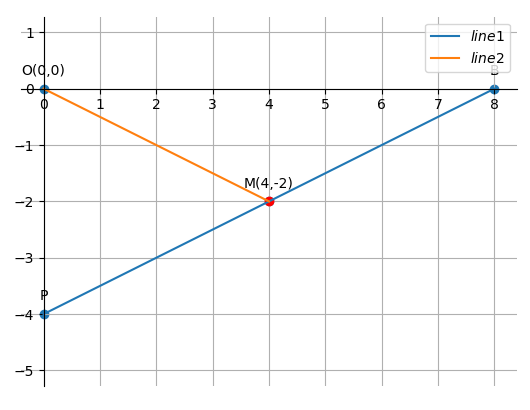
\includegraphics[width=0.75\columnwidth]{chapters/11/10/1/5/figs/line.png}
 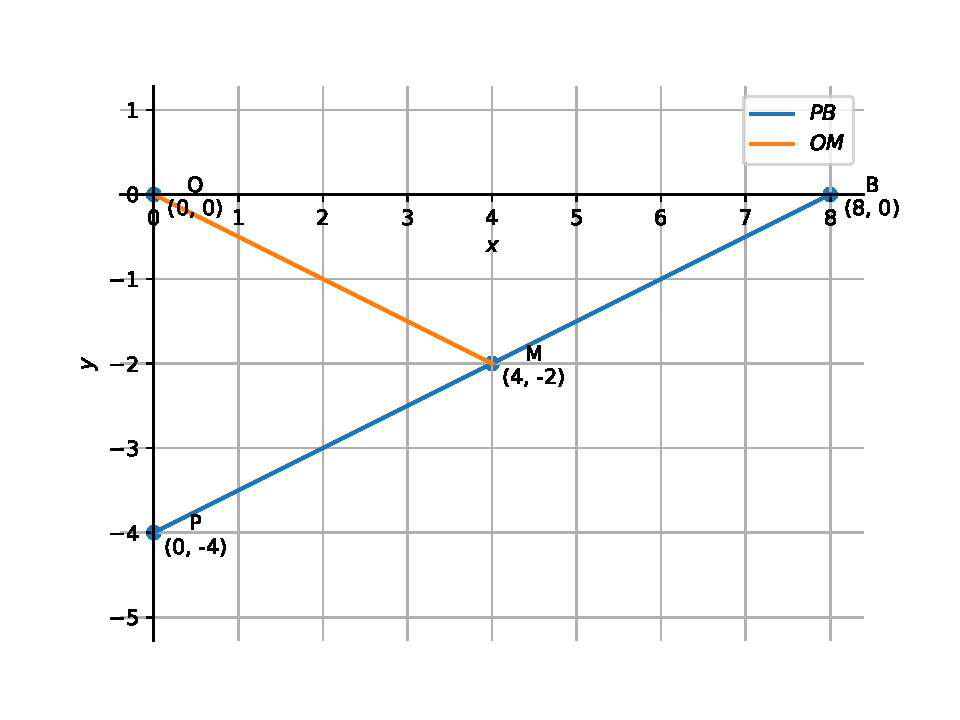
\includegraphics[width=0.75\columnwidth]{chapters/11/10/1/5/figs/fig.pdf}
		\caption{}
		\label{fig:11/10/1/5}
  	\end{figure}

\item A line passes through $A(x_1,y_1)$ and $B(h,k)$. If slope of the line is m, show that $(k-y_1)=m(h-x_1)$.
\label{chapters/11/10/1/12}
\\
\solution 
The direction vector
\begin{align}
	\vec{B}-\vec{A}
	=
	\myvec{
  h-x_1\\
  k-y_1
  }
   \equiv
	\myvec{
1\\
	\frac{ k-y_1}{h-x_1}
  }
  \\
	\implies m = 
	\frac{ k-y_1}{h-x_1},
\end{align}
yielding the desired result.

\item
Show that the line through the points \brak{4,7,8},\brak{2,3,4} is parallel to the line through the points \brak{-1,-2,1},\brak{1,2,5}.
	\label{12.11.2.3}
\\
\solution
	Show that the line through the points \brak{4,7,8},\brak{2,3,4} is parallel to the line through the points\brak{-1,-2,1},\brak{1,2,5}.

\textbf{Solution :}
For line passing through \brak{4,7,8},\brak{2,3,4},the direction vector,\begin{align}
    \vec{m_1}&=\myvec{-2\\-4\\-4}
\end{align}
For line passing through \brak{-1,-2,1},\brak{1,2,5},the direction vector,\begin{align}
    \vec{m_2}&=\myvec{2\\4\\4}
\end{align}
Therefore,the lines are parallel to each other.

\item For given vectors, $\vec{a}=2\hat{i}-\hat{j}+2\hat{k}$ and $\vec{b}=-\hat{i}+\hat{j}-\hat{k}$ , find the unit vector in the
direction of the vector $\vec{a}+\vec{b}$.
        \label{prob:12/10/2/9}
\\
    \solution 
		\begin{align}
	\because \vec a + \vec b = \myvec{ 2\\-1\\2 } + \myvec{ -1\\1\\-1 },
= \myvec{ 1\\0\\1 },
\\
	\norm{\vec a + \vec b } = \sqrt{2}
	\\
	\implies \frac{\vec a + \vec b }{\norm{\vec a + \vec b }} = \frac{1}{\sqrt{2}}\myvec{ 1\\0\\1 }
\end{align}
which, from  \eqref{eq:unit-vec} is the desired the unit vector.
		





\item Find a vector of magnitude 5 units, and parallel to the resultant of the vectors $\vec{a}=2\hat{i}+3\hat{j}-\hat{k}$ and $\vec{b}=\hat{i}-2\hat{j}+\hat{k}$.\\
\item If $\vec{a}=\hat{i}+\hat{j}+\hat{k}, \vec{b}=2\hat{i}-\hat{j}+3\hat{k}$ and $\vec{c}=\hat{i}-2\hat{j}+\hat{k}$, find a unit vector parallel to the vector $2\vec{a}-\vec{b}+3\vec{c}$.\\
	\solution
		\begin{align}
2\vec{a}-\vec{b}+3\vec{c}=\myvec{3\\-3\\2}
\implies
\frac{2\vec{a}-\vec{b}+3\vec{c}}{\norm{2\vec{a}-\vec{b}+3\vec{c}}}
=\frac{1}{\sqrt{22}}\myvec{3\\-3\\2}
\end{align}


\item Find a vector in the direction of vector $5\hat{i}-\hat{j}+2\hat{k}$ which has magnitude 8 units.
        \label{prob:12/10/2/10const}
   \\ 
    \solution 
		Let the required vector be 
    \begin{align}
c\myvec{5\\-1\\2}.
    \end{align}
    From the given information, 
    \begin{align}
        \norm{c\myvec{5\\-1\\2\\}} =  8 \\
	    \implies \abs{c} = \frac{4\sqrt{30}}{15}
        \label{eq:12/10/2/10const}
    \end{align}


\item Find the unit vector in the direction of the vector $\vec{a}=\hat{i}+\hat{j}+2\hat{k}$.
\item Find the unit vector in the direction of vector $\overrightarrow{PQ}$ , where $\vec{P}$ and $\vec{Q}$ are the points
(1, 2, 3) and (4, 5, 6), respectively.
	\item 
Find a vector of magnitude 5 units, and parallel to the resultant of the vectors $\vec{a} = 2\hat{i}+3\hat{j}-\hat{k}$ and $\vec{b} = \hat{i}-2\hat{j}+\hat{k}$.
\\
\solution
		\begin{align}
\because     \Vec{a}=\myvec{
        2\\3\\-1
    },\Vec{b}=\myvec{
        1\\-2\\1
    }\\
	\vec{a}+\vec{b}=\myvec{
        3\\1\\0
    }
    \implies
	\norm{\vec{a}+\vec{b}}=\sqrt{10}
\end{align}
From problem
        \ref{prob:12/10/2/9},
the unit vector in the direction of 
${\vec{a}+\vec{b}}$
is
\begin{align}
	\frac{{\vec{a}+\vec{b}}}{\norm{\vec{a}+\vec{b}}}
=\frac{1}{\sqrt{10}}\myvec{
        3\\1\\0
    }
\end{align}
The desired vector can then be expressed as
\begin{align}
\pm\frac{5}{\sqrt{10}}\myvec{
        3\\1\\0
    }
\end{align}


	\item If a line makes angles $90\degree,135\degree,45\degree$ with x,y and z-axis respectivly. Find its direction cosines.
		\\
		\solution
				From \eqref{eq:dir-vec-3d},
the direction vector is
\begin{align}
\vec{A}=\myvec{\cos 90\degree\\ \cos 135\degree\\ \cos 45\degree}=\myvec{0\\-\frac{1}{\sqrt{2}}\\ \frac{1}{\sqrt{2}}}
\end{align}

\item Find the direction cosines of the vector joining the points $\vec{A}$ (1, 2, –3) and
$\vec{B}$(–1, –2, 1), directed from $\vec{A}$ to $\vec{B}$.
	\\
    \solution 
		The unit vector  in the direction of AB is 
\begin{align}
	\frac{\vec{B}-\vec{A}}{\norm{\vec{B}-\vec{A}}}
	= \frac{1}{3}{\myvec{-1\\-2\\2}}
\end{align}
and the direction cosines are the elements of the above vector.

\item Show that the vector $\hat{i}+\hat{j}+\hat{k}$ is equally inclined to the axes OX, OY and OZ.
	\\
\solution
		Since all entries of the given vector 
\begin{align}
\myvec{1\\1\\1}
\end{align}
are equal, it is equally inclined to the axes.

\item If a line has the direction ratios –18, 12, –4, then what are its direction cosines?
		\\
		\solution
		Let
\begin{align}
	\vec{A} =\myvec{-18\\12\\-4}
\end{align}
Then the unit direction vector of the line is
\begin{align}
		\frac{\vec{A}}{\norm{\vec{A}}} =
\myvec{\frac{-9}{11}\\[2pt] \frac{6}{11}\\[2pt] \frac{-2}{11}}
\end{align}

	\item Find the direction cosines of the sides of a triangle whose vertices are $\myvec{3\\ 5\\-4 }$, $\myvec{ -1\\1 \\2 }$ and $\myvec{-5 \\-5 \\-2 }$.
		\\
		\solution
		Let the vertices be
\begin{align}
\vec{A} = \myvec{3\\5\\-4},
\vec{B} = \myvec{-1\\1\\2},
\vec{C} = \myvec{-5\\-5\\-2}
\end{align}
%
The direction vectors of the sides are,
\begin{align}
\vec{A} - \vec{B} = \myvec{4\\4\\-6} = \vec{m_1},
\vec{B} - \vec{C} = \myvec{4\\6\\4} = \vec{m_2}, 
\\
\vec{C} - \vec{A} = \myvec{-8\\-10\\2} =\vec{m_3},
\end{align}
%
The corresponding unit vectors are then obtained as
\begin{align}
 \myvec{ \frac{2}{\sqrt{17}} \\[1pt] \frac{2}{\sqrt{17}} \\[1pt] \frac{-3}{\sqrt{17}} },
 \myvec{ \frac{2}{\sqrt{17}} \\[1pt] \frac{3}{\sqrt{17}} \\[1pt] \frac{2}{\sqrt{17}} }, 
 \myvec{ \frac{-4}{\sqrt{42}} \\[1pt] \frac{-5}{\sqrt{42}} \\[1pt] \frac{1}{\sqrt{42}} } 
\end{align}

\item Find the direction cosines of the vector $\hat{i}+2\hat{j}+3\hat{k}$.
	\\
    \solution 
		The unit vector in the direction of the given vector is 
\begin{align}
	\vec{A} =\frac{1}{\sqrt{14}}\myvec{1\\2\\3}
\end{align}

    \item Find the direction cosines of a line which makes equal angles with the coordinate
    axes.
		\\
		\solution
		Let $\alpha$ be the angle made by the line with the axes.  The unit direction vector can be expressed as
    \begin{align}
	    \vec{x} &= \myvec{\cos\alpha\\\cos\alpha\\\cos\alpha} 
	\implies
	    \norm{\vec{x}}  = 1
	\\
	    \text{or, }\cos\alpha &= \frac{1}{\sqrt{3}}
    \end{align}
    Thus the unit direction vector  of the given line is 
    \begin{align}
	    \vec{x} = \frac{1}{\sqrt{3}} \myvec{1 \\ 1 \\ 1} 
\end{align}
    

\item Write down a unit vector in XY-plane, making an angle of 30$\degree$ with the positive direction of x-axis.\\
\item the unit vector normal to the plane $x+2y+3z-6=0$ is $\dfrac{1}{\sqrt{14}}\hat{i} + \dfrac{2}{\sqrt{14}}\hat{j} + \dfrac{3}{\sqrt{14}}\hat{k}$.
\end{enumerate}
